\chapter{Statistical Learning Theory e VC-dimension}\label{ch-12}

Dopo le tecniche empiriche di validazione, si torna alla \textbf{stima
analitica} dell'errore atteso (di validazione, per la model selection, o
di test, per l'assessment), introdotta in
\href{04\%20-\%20Generalizzazione\%20e\%20validazione\%20(introduzione)}{04
- Generalizzazione e validazione (introduzione)}. Questa lezione
definisce formalmente la \textbf{VC-dimension}, la calcola per alcune
classi di ipotesi, presenta il bound della SLT e il principio della
\textbf{Structural Risk Minimization} (SRM), che porterà alle SVM.

Ricordiamo le alternative per stimare l'errore:

\begin{itemize}
\tightlist
\item
  \textbf{analitiche}: AIC, BIC (limitati ai modelli lineari nei
  parametri), MDL, \textbf{SRM con VC-dimension};
\item
  \textbf{per ricampionamento}: cross-validation, bootstrap.
\end{itemize}

\section{La VC-dimension}\label{la-vc-dimension}

Per ottenere un bound analitico dobbiamo valutare lo spazio delle
ipotesi \(H\). Serve una misura della sua \textbf{complessità}
(capacità, potere espressivo, flessibilità) che funzioni anche per \(H\)
\textbf{infiniti} (come i modelli lineari, con pesi reali): non si può
quindi usare \(|H|\). L'idea di Vapnik e Chervonenkis è misurare invece
\textbf{il numero di istanze distinte che \(H\) riesce a discriminare
completamente}.

Intuitivamente, nel caso della classificazione: \emph{quanto \(H\)
riesce a discriminare dei punti?} Qual è il \textbf{numero massimo di
punti che si possono classificare correttamente, senza errori, per tutte
le possibili etichettature}?

\subsection{Shattering}\label{shattering}

Sia \(X\) lo spazio delle istanze, con \(N\) punti (attenzione: \(N\)
qui è il numero di istanze considerate, che può essere diverso dal
numero di dati \(l\)), e sia \(H\) lo spazio delle ipotesi per la
classificazione binaria.

\begin{itemize}
\tightlist
\item
  Esistono \(2^N\) possibili \textbf{dicotomie} (partizioni, o
  etichettature dei punti con \(-1\) o \(+1\)).
\item
  Una dicotomia è \textbf{rappresentata} in \(H\) se esiste un'ipotesi
  \(h \in H\) che la realizza.
\end{itemize}

\begin{boxdefinition}{Shattering (frammentazione)}

\(H\) \textbf{frammenta} (\emph{shatters}) \(X\) se e solo se \(H\) può
rappresentare \textbf{tutte} le possibili dicotomie su \(X\) (con errore
zero): per ogni possibile etichettatura dei punti esiste un'ipotesi
\(h \in H\) consistente con essa.

\end{boxdefinition}

\begin{boxexample}{Tre punti nel piano e le rette}

Consideriamo 3 punti in \(\mathbb{R}^2\) e come \(H\) l'insieme delle
rette,
\(h(\mathbf{x}) = \operatorname{sign}(\mathbf{w}^T\mathbf{x} + w_0)\).
Una specifica dicotomia (ad esempio due punti a \(-1\) e uno a \(+1\)) è
rappresentabile se esiste una retta che separa correttamente i punti. Le
dicotomie possibili sono \(2^3 = 8\).

\end{boxexample}

\begin{figure}[htbp]
\centering
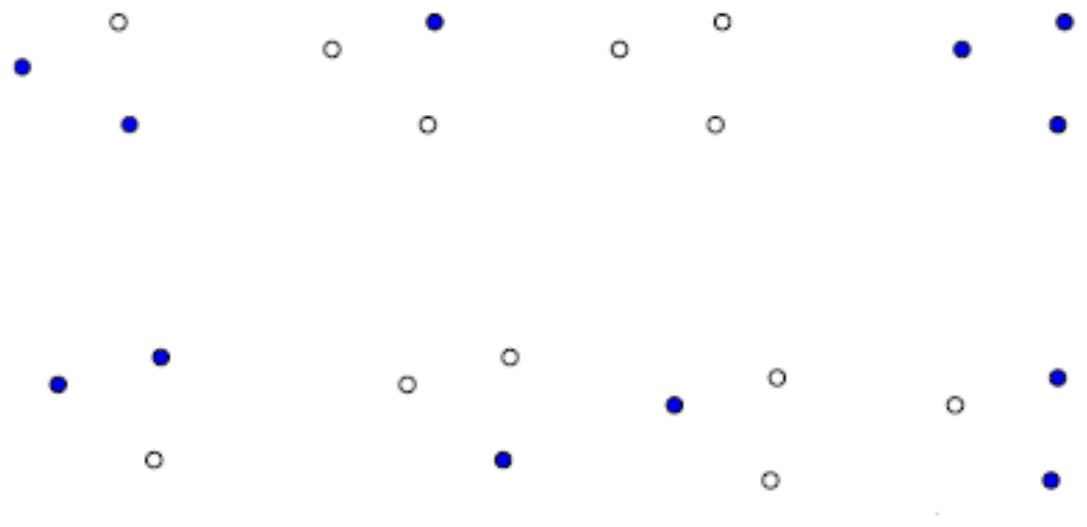
\includegraphics[width=0.71\linewidth,height=0.42\textheight,keepaspectratio]{images/12-slt_dicotomie.png}
\caption{Tutte le \(2^N = 8\) dicotomie di 3 punti in \(\mathbb{R}^2\).}
\end{figure}

\begin{figure}[htbp]
\centering
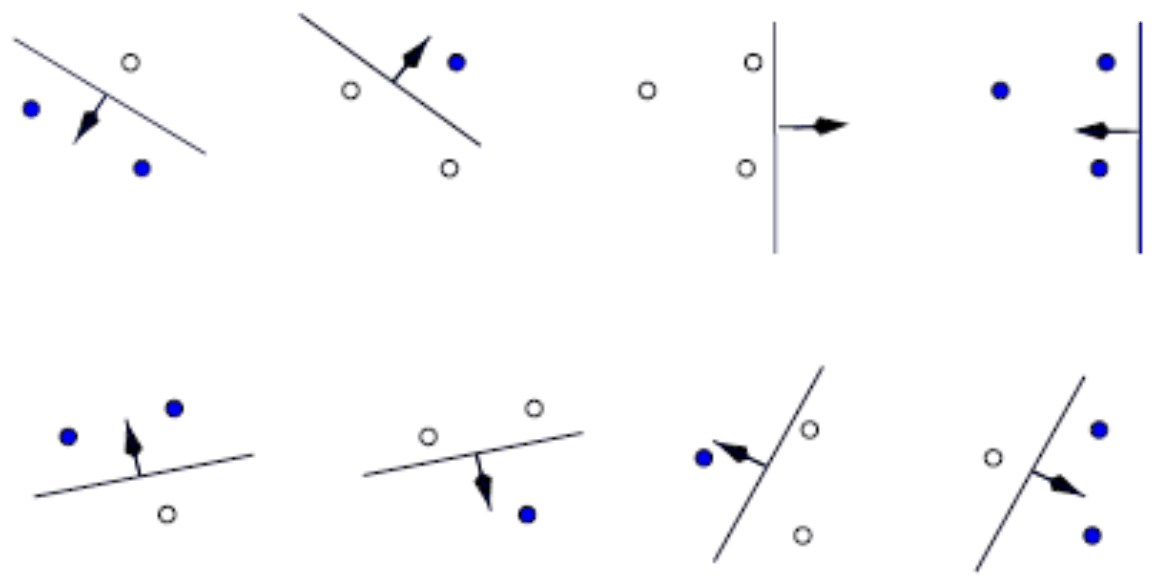
\includegraphics[width=0.71\linewidth,height=0.42\textheight,keepaspectratio]{images/12-slt_shattering.png}
\caption{Per ogni dicotomia esiste una retta separatrice: le funzioni lineari
frammentano questi 3 punti.}
\end{figure}

\subsection{Definizione di
VC-dimension}\label{definizione-di-vc-dimension}

\begin{boxdefinition}{VC-dimension}

La \textbf{VC-dimension} di una classe di funzioni \(H\) è la
\textbf{cardinalità massima di un insieme di punti} (in una qualche
configurazione) di \(X\) che può essere frammentato da \(H\).
\(VC(H) = p\) significa che:

\begin{itemize}
\tightlist
\item
  \(H\) frammenta \textbf{almeno un} insieme (configurazione) di \(p\)
  punti;
\item
  \(H\) \textbf{non} frammenta \textbf{nessun} insieme di \(p+1\) punti.
\end{itemize}

Se si possono frammentare insiemi di dimensione arbitrariamente grande,
\(VC(H) = \infty\).

\end{boxdefinition}

Attenzione all'asimmetria: per il limite inferiore basta \textbf{una}
configurazione frammentabile; per il limite superiore bisogna mostrare
che \textbf{nessuna} configurazione di \(p+1\) punti è frammentabile.

\subsection{VC-dimension degli iperpiani nel
piano}\label{vc-dimension-degli-iperpiani-nel-piano}

\begin{itemize}
\tightlist
\item
  \textbf{\(VC(H) \ge 3\)}: l'abbiamo appena mostrato con 3 punti non
  allineati. Non tutte le configurazioni di 3 punti sono frammentabili:
  tre punti \textbf{allineati} con quello centrale di classe diversa non
  sono linearmente separabili. Ma basta \textbf{una} configurazione
  frammentabile.
\item
  \textbf{\(VC(H) < 4\)}: dati 4 punti qualsiasi nel piano, si possono
  sempre tracciare i 6 segmenti che li collegano a coppie, e due di
  questi si incrociano (se i 4 punti formano un quadrilatero convesso
  sono le diagonali; se uno è dentro il triangolo degli altri, si
  sceglie l'etichettatura con il punto interno di classe diversa).
  Mettendo nella stessa classe i punti collegati dai segmenti che si
  incrociano, non si possono separare linearmente: è lo \textbf{XOR}.
\end{itemize}

\begin{figure}[htbp]
\centering
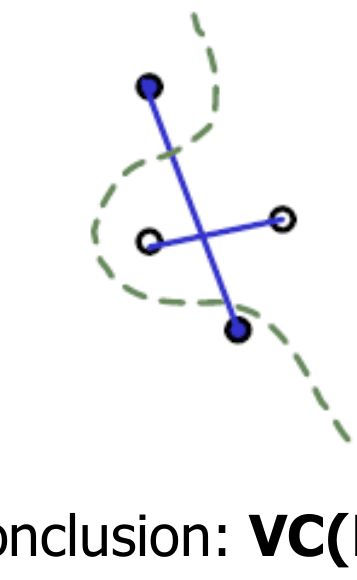
\includegraphics[width=0.31\linewidth,height=0.42\textheight,keepaspectratio]{images/12-slt_quattro-punti.png}
\caption{Con 4 punti esiste sempre un'etichettatura di tipo XOR non separabile da
una retta.}
\end{figure}

Conclusione: \textbf{\(VC(H) = 3\)} per gli iperpiani (LTU) in
\(\mathbb{R}^2\).

\begin{boxtheorem}{VC-dimension degli iperpiani}

La VC-dimension della classe degli iperpiani separatori (LTU) in uno
spazio \(n\)-dimensionale è \(n + 1\).

\end{boxtheorem}

È un limite superiore: vincolando il modello (ad esempio limitando la
norma dei pesi, come si vedrà nelle SVM) può diminuire.

\subsection{Altri esempi}\label{altri-esempi}

{\def\LTcaptype{none} % do not increment counter
\begin{longtable}[]{@{}
  >{\raggedright\arraybackslash}p{(\linewidth - 2\tabcolsep) * \real{0.5000}}
  >{\raggedright\arraybackslash}p{(\linewidth - 2\tabcolsep) * \real{0.5000}}@{}}
\toprule\noalign{}
\begin{minipage}[b]{\linewidth}\raggedright
Classe \(H\)
\end{minipage} & \begin{minipage}[b]{\linewidth}\raggedright
VC-dim
\end{minipage} \\
\midrule\noalign{}
\endhead
\bottomrule\noalign{}
\endlastfoot
Rette in \(\mathbb{R}\) (soglie, \(\operatorname{sign}(w_1x + w_0)\)) &
2 \\
Intervalli su \(\mathbb{R}\) & 2 \\
Cerchi centrati nell'origine in 2D,
\(\operatorname{sign}(\mathbf{x}\cdot\mathbf{x} - b)\) & 1 \\
Cerchi centrati nell'origine,
\(\operatorname{sign}(k\,\mathbf{x}\cdot\mathbf{x} - b)\) & 2 \\
Cerchi (raggio e centro liberi) in 2D & 3 \\
Cerchi (raggio fisso, centro libero) in 2D & 3 \\
\end{longtable}
}

(Per i cerchi centrati nell'origine con un solo parametro \(b\), il
cerchio include i punti vicini all'origine: con due punti a distanze
diverse non si può etichettare ``+'' il più lontano e ``−'' il più
vicino. Aggiungendo \(k\) si può invertire l'interno e l'esterno, e la
VC-dim sale a 2.)

La VC-dimension può essere difficile da calcolare per modelli con
parametri non lineari.

\subsection{VC-dimension e numero di
parametri}\label{vc-dimension-e-numero-di-parametri}

La VC-dimension è il numero di parametri liberi? \textbf{Sono legati ma
non coincidono}:

\begin{itemize}
\tightlist
\item
  nell'esempio dei cerchi, classi con lo \textbf{stesso} numero di
  parametri hanno VC-dim diverse, e viceversa;
\item
  si possono aggiungere parametri \textbf{ridondanti} senza cambiare
  nulla;
\item
  esistono modelli con \textbf{un solo parametro e VC-dim infinita}
  (l'esempio classico è \(\operatorname{sign}(\sin(\alpha x))\), che con
  un \(\alpha\) abbastanza grande frammenta qualsiasi insieme di punti
  opportunamente scelti);
\item
  per il \textbf{nearest neighbor} la VC-dim è \textbf{infinita} (il
  1-NN classifica correttamente qualunque etichettatura del training
  set).
\end{itemize}

\section{Il bound analitico sul
rischio}\label{il-bound-analitico-sul-rischio}

Sia \(N\) il numero di dati (\(l\)).

\begin{boxtheorem}{VC-bound}

Con probabilità almeno \(1 - \delta\), per ogni \(h \in H\) (con
\(VC < N\)): \[
R[h] \;\le\; R_{emp}[h] + \varepsilon(VC, N, \delta),
\] dove il membro destro è il \textbf{rischio garantito} e
\(\varepsilon\) è la \textbf{VC-confidence}. Ad esempio, per la loss
0/1: \[
\varepsilon(VC, N, \delta) = \sqrt{\frac{VC\left(\ln\frac{2N}{VC} + 1\right) - \ln\frac{\delta}{4}}{N}}.
\]

\end{boxtheorem}

Esistono formulazioni diverse per diverse classi di funzioni e task.
L'interpretazione è quella già vista: \(\varepsilon \to 0\) al crescere
di \(N\), \(\varepsilon\) cresce con la VC-dim, e il bound su \(R\) ha
un andamento a U al crescere della VC-dim.

Nella formula si vede bene: \(\varepsilon\) dipende essenzialmente dal
rapporto \(VC/N\) (a meno di logaritmi). Raddoppiare i dati ha lo stesso
effetto di dimezzare la complessità.

Il bound permette di \textbf{stimare l'errore sui dati futuri} basandosi
solo sull'errore di training e sulla VC-dimension di \(H\), e la
VC-confidence si può calcolare \textbf{prima} dell'apprendimento.

\begin{boxwarning}{Bound ``nel caso peggiore''}

I bound risultanti sono \emph{worst case}: devono valere per tutte le
funzioni e tutti i training set, tranne una frazione \(\delta\). Per
questo sono spesso molto larghi.

\end{boxwarning}

\begin{boxtip}{Una conseguenza pratica}

Per molte classi ragionevoli (es. approssimatori lineari) la VC-dim è
\textbf{lineare nel numero di parametri liberi}. Quindi, per apprendere
``bene'', serve un numero di esempi \textbf{lineare nella VC-dimension}
(e quindi, in questo caso, nel numero di parametri). È una spiegazione
teorica di euristiche pratiche come ``servono almeno \(k\) esempi per
parametro''.

\end{boxtip}

\section{Structural Risk
Minimization}\label{structural-risk-minimization}

La \textbf{SRM} usa la VC-dimension come parametro di controllo per
minimizzare il bound sul rischio. Assumendo VC-dim finite, si definisce
una \textbf{struttura annidata} di spazi delle ipotesi ordinati per
VC-dim: \[
H_1 \subseteq H_2 \subseteq \dots \subseteq H_n, \qquad VC(H_1) \le \dots \le VC(H_n).
\]

Esempi di strutture:

\begin{itemize}
\tightlist
\item
  reti neurali con numero crescente di \textbf{unità nascoste} (circa),
  ma anche con numero crescente di \textbf{epoche} (sappiamo che conta
  anche la grandezza dei pesi: la rete è uno spazio di dimensione
  variabile);
\item
  polinomi di \textbf{grado} \(M\) crescente;
\item
  valori crescenti di \(c\), dove \(\|\mathbf{w}\| < c\) per la
  \textbf{regolarizzazione} (o equivalentemente controllato da
  \(\lambda\));
\item
  alberi di decisione con numero crescente di nodi (circa).
\end{itemize}

Gli \textbf{iperparametri importanti} sono proprio quelli legati alla
VC-dimension.

\subsection{SRM per la model
selection}\label{srm-per-la-model-selection}

Al crescere della VC-dim l'errore empirico (di training)
\textbf{diminuisce} e la VC-confidence \textbf{aumenta}. La SRM cerca il
compromesso sul bound \[
R \le R_{emp} + \varepsilon(1/l, VC, 1/\delta),
\] cioè sceglie il modello \(h\) con il \textbf{miglior bound sul
rischio vero}.

\begin{figure}[htbp]
\centering
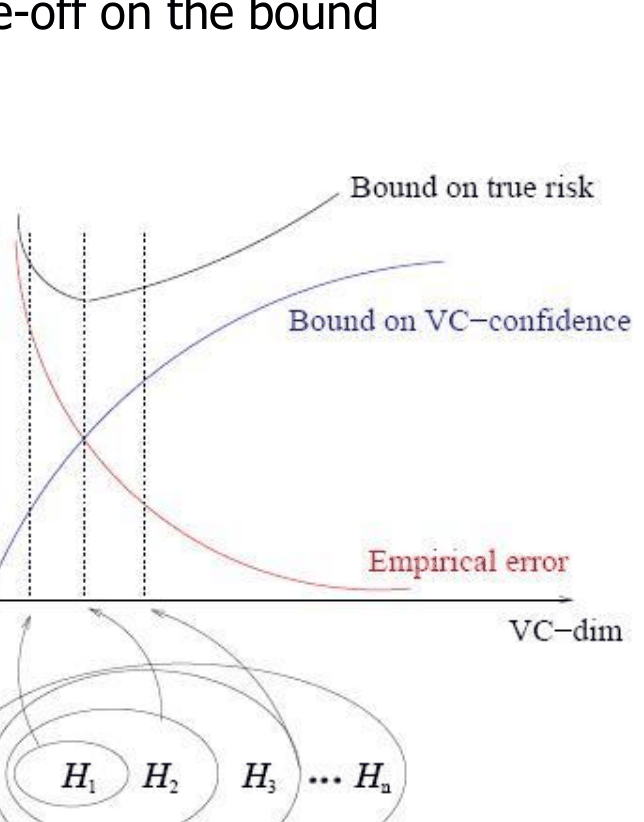
\includegraphics[width=0.46\linewidth,height=0.42\textheight,keepaspectratio]{images/12-slt_srm.png}
\caption{Structural Risk Minimization: su una struttura annidata di spazi delle
ipotesi si sceglie quello che minimizza il bound sul rischio.}
\end{figure}

\begin{figure}[htbp]
\centering
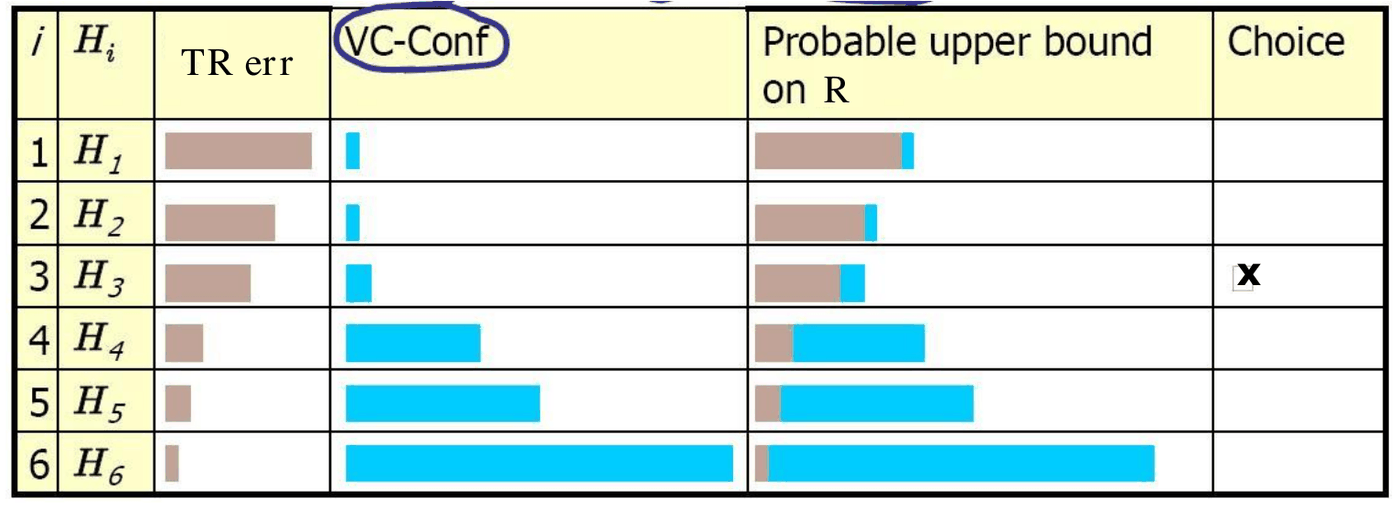
\includegraphics[width=0.86\linewidth,height=0.42\textheight,keepaspectratio]{images/12-slt_srm-tabella.png}
\caption{Model selection con SRM: si sceglie \(H_3\), con il minimo bound
probabile su \(R\).}
\end{figure}

\begin{boxwarning}{Attenzione}

La VC-confidence può essere \textbf{molto conservativa}: anche centinaia
di volte più grande dell'effetto di overfitting osservato empiricamente.

\end{boxwarning}

\subsection{A cosa serve il bound}\label{a-cosa-serve-il-bound}

\begin{itemize}
\tightlist
\item
  Fornisce un \textbf{fondamento teorico} al ML basato su principi,
  indipendente dai dettagli del modello o dell'algoritmo; evidenzia il
  ruolo del \textbf{controllo della complessità}; mostra che la scelta
  ottima della complessità (sulla struttura) minimizza il rischio
  atteso: è il \textbf{principio induttivo della SRM}.
\item
  Come \textbf{stima dell'errore predittivo} è usato raramente:

  \begin{itemize}
  \tightlist
  \item
    può essere molto largo, ma resta utile per la \textbf{model
    selection}, dove conta la \textbf{dimensione relativa} (il
    \emph{ranking}) degli errori;
  \item
    è un upper bound probabilistico valido per \textbf{tutte} le
    funzioni della classe, quindi si può cercare nella classe;
  \item
    è difficile calcolare la VC-dim di classi specifiche;
  \item
    il bound grezzo (troppo pessimistico) può non essere adeguato per
    una valutazione affidabile dell'errore di generalizzazione
    (\textbf{model assessment}); si stanno sviluppando bound più
    stretti.
  \end{itemize}
\item
  Indica una direzione per sviluppare \textbf{nuovi modelli} guidati
  dalla SRM, verso approcci basati su principi e meno su tentativi
  empirici.
\end{itemize}

\subsection{Due approcci pratici alla
SRM}\label{due-approcci-pratici-alla-srm}

\begin{enumerate}
\def\labelenumi{\arabic{enumi}.}
\tightlist
\item
  \textbf{Fissare la struttura/complessità} (e quindi la VC-confidence)
  e \textbf{minimizzare l'errore di training}. Si può usare con le reti
  neurali. Le euristiche di addestramento possono già realizzare una SRM
  \textbf{implicita} (early stopping, \ldots); oppure si realizza la SRM
  con la \textbf{regolarizzazione di Tikhonov}, minimizzando una loss
  \(R_{emp}\) + termine di complessità, che considera entrambi i
  termini.
\item
  \textbf{Fissare l'errore di training} e \textbf{minimizzare
  automaticamente la VC-confidence}. Come? È l'idea delle \textbf{SVM}
  (\href{13\%20-\%20Support\%20Vector\%20Machines}{13 - Support Vector
  Machines}).
\end{enumerate}

\begin{boxabstract}{Sintesi}

La \textbf{VC-dimension} misura la capacità di \(H\) come il massimo
numero di punti che \(H\) riesce a frammentare (classificare
correttamente per ogni etichettatura). Per gli iperpiani in
\(\mathbb{R}^n\) vale \(n+1\); non coincide con il numero di parametri
(può essere infinita con un solo parametro, ed è infinita per il NN). Il
\textbf{VC-bound} \(R \le R_{emp} + \varepsilon(VC, N, \delta)\) lega
rischio, errore di training, complessità e numero di dati. La
\textbf{SRM} sceglie, in una struttura annidata di spazi, quello che
minimizza il bound. I bound sono spesso larghi, ma forniscono il
fondamento teorico del controllo della complessità.

\end{boxabstract}

\begin{boxquestion}{Possibili domande d'esame}

\begin{itemize}
\tightlist
\item
  Definire shattering e VC-dimension.
\item
  Dimostrare che la VC-dim delle rette nel piano è 3.
\item
  La VC-dim coincide con il numero di parametri liberi? Esempi.
\item
  Scrivere il VC-bound e interpretarne i termini.
\item
  Cos'è la Structural Risk Minimization? Esempi di strutture annidate.
\item
  Quali sono i limiti pratici del bound? A cosa serve comunque?
\end{itemize}

\end{boxquestion}
